% Chapter 2

\chapter{Experimental methods and results} 

% \label{ch:mandelbrotpercolation} % For referencing the chapter elsewhere, use \autoref{ch:introduction} 

%----------------------------------------------------------------------------------------

%----------------------------------------------------------------------------------------

To experimentally verify the results described above, we ran more than \textbf{3 billion simulations}, generating approximately \textbf{250GB} of data. The code that used to run the simulation and to extract the statistics is available in Github, see Appendix 1 for more details. The full data is also available, see Appendix 2. 


\section{2D lattice simulation}


We used a $L \times L$ square, periodic lattice, which is topologically equivalent to a torus. Each node has four neighbours: one above it, one to the right, one below, and one to the left. The periodicity is represented by the fact that the right neighbors of the nodes in the rightmost column are the nodes in the leftmost column. Similarly, the left neighbours of the leftmost column are the nodes in the rightmost column, the top neighbours of the topmost row are the nodes in the bottom-most row, and the bottom neighbours of the bottom-most row are nodes in the topmost row.

Each node can be in one of two states: dead or alive. Initially, all nodes are in the alive state. With probability $p$, we change state of each individual node to dead. We then compute and store the set of clusters found in the lattice. A cluster is a set of connected nodes sharing the same state. 

Each cluster can either be a finite or infinite. Since the lattice is periodic, a cluster is considered infinite if its 1D extension in either direction is greater than or equal to the size of the lattice $L$. Otherwise, it is a finite cluster. In other words, we imagine a bounding box around each cluster, and if at least of the dimensions of the box is greater than or equal to $L$, the cluster is infinite. 

We generated around 3000 lattices for each pair $(p, L)$, with $p$ ranging from 0 to 1 (with a higher density near the critical points) and $L$ ranging from 16 to 1024.


\section{Percolation probability}

A lattice has percolated if it contains at least one infinite cluster. For each $(p, L)$, we count the number of percolating lattices and divide by the total number of lattices to compute the percolation probability.

In \autoref{fig:sec3_perc_prob_1}, we plot the percolation probability against the occupation probability $p$ for various lattice sizes.


\begin{figure}[H]
  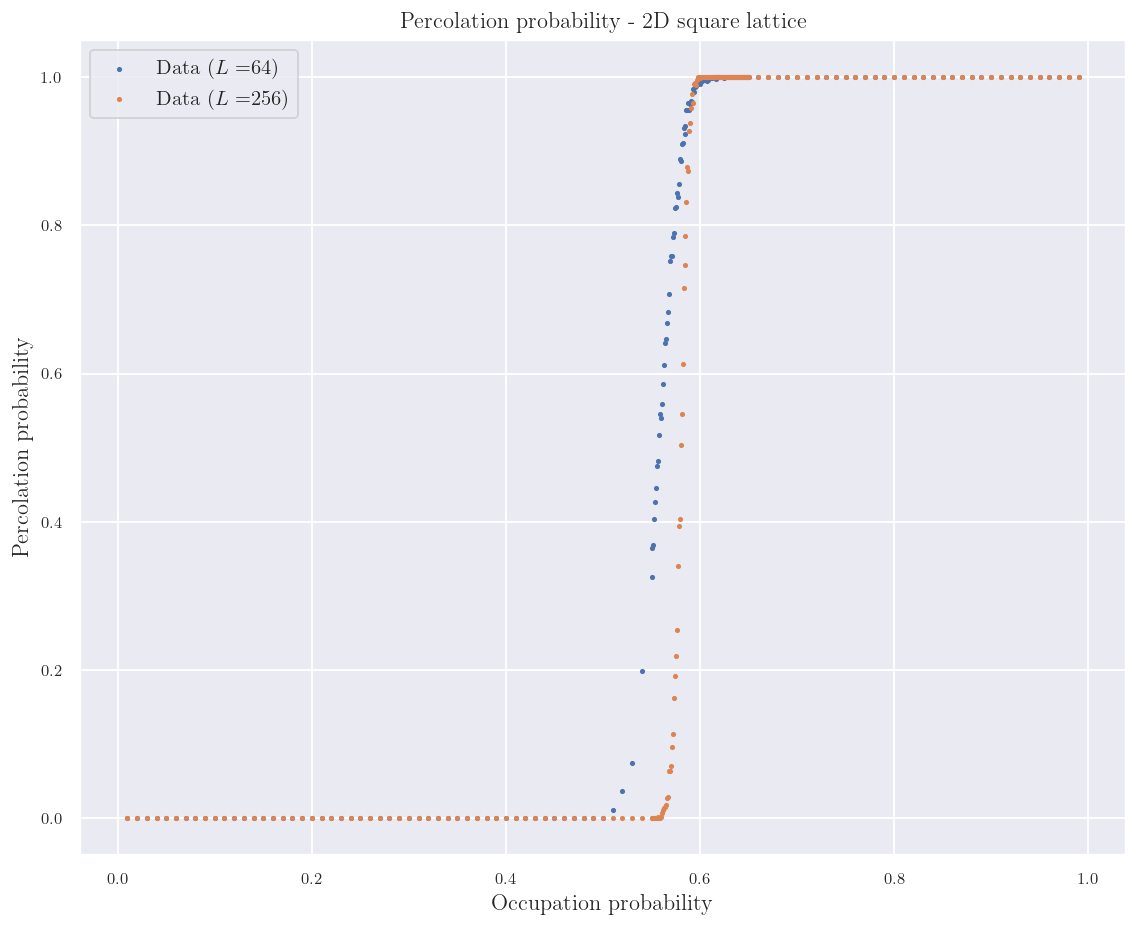
\includegraphics[width=\linewidth]{Images/sec3_perc_prob_1.png}
  \caption{Percolation probability curve for various lattice sizes}
  \label{fig:sec3_perc_prob_1}
\end{figure}

By visual inspection, we can hypothesize that the curve is a hyperbolic tangent curve: 

$$ 
y(x) = \tanh(x)
$$

We can shift and scale this function so that it's centered at $x=\beta$, and such that it's domain matches our data, i.e. $\mathcal{D}(y) = \left[ 0, 1 \right]$. We'd also like a parameter that controls how steep the transition is between $y=0$ and $y=1$ - this can be done by scaling $x$ by a multiplicative factor $\alpha$. The function becomes

$$ 
y(x) = \frac{\tanh(\alpha(x - \beta)) + 1}{2}
$$ 

In \autoref{fig:sec3_perc_prob_2}, we can see the the fitted data points. \autoref{table:sec3_tahn_fit_parameters} contains the precise values.


\begin{figure}[H]
  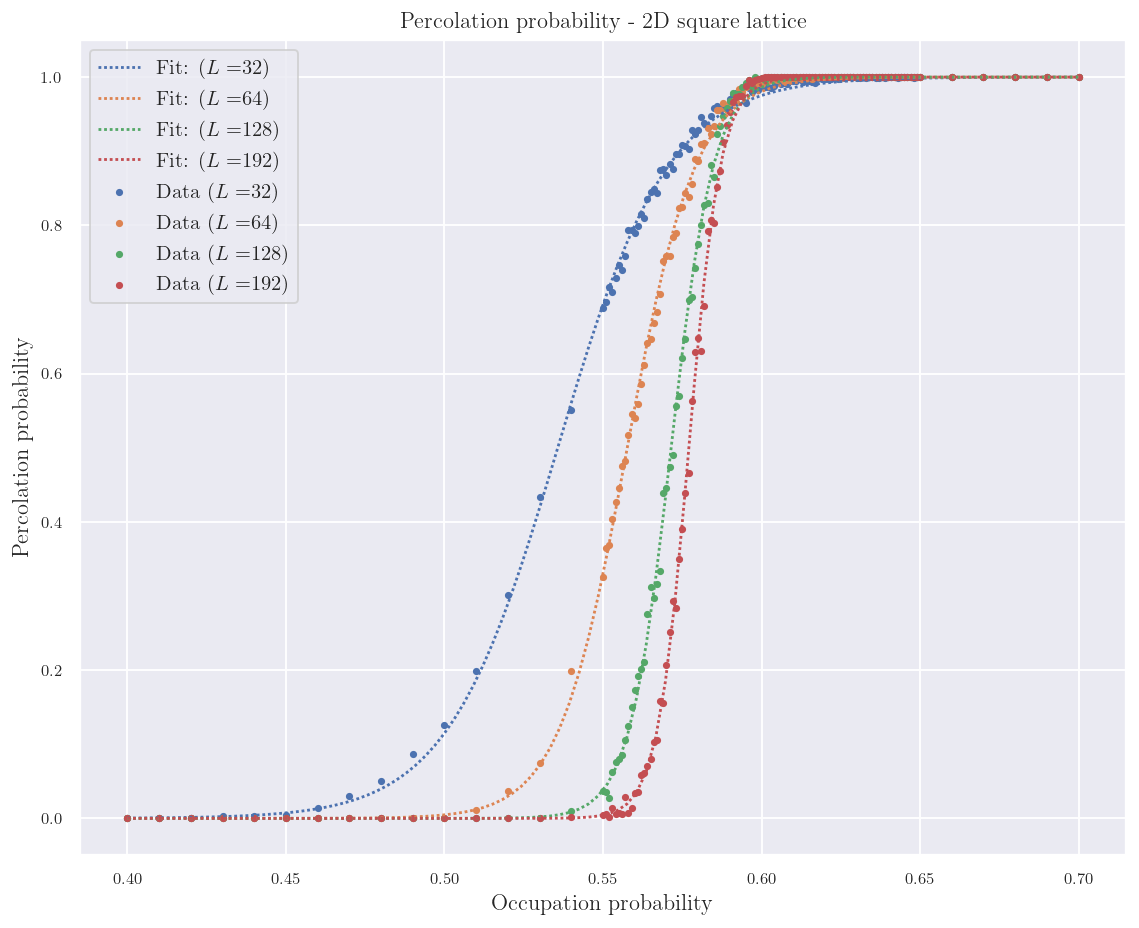
\includegraphics[width=\linewidth]{Images/sec3_perc_prob_2.png}
  \caption{Percolation probability curve zoomed in, along with the hyperbolic tangent least squares fit.}
  \label{fig:sec3_perc_prob_2}
\end{figure}

We notice that the the bigger the lattice, the faster it jumps from $y=0$ to $y=1$. This is consistent with the widely known fact that as L increases, i.e. in the limit $L \rightarrow \infty $, the transition becomes a step function at $p = p_c$. 

Another interesting fact to notice is that with the structure of the function we're fitting, $\beta$ represents the point at which the percolation probability first reaches $\frac{1}{2}$.

These two observations suggest that studying the behaviour of $\alpha$ and $\beta$ as a function of the lattice size $L$ might be interesting. We can see the results obtained in \autoref{fig:sec3_perc_prob_3}, along with a so called finite-size scaling analysis.

\begin{figure}[H]
  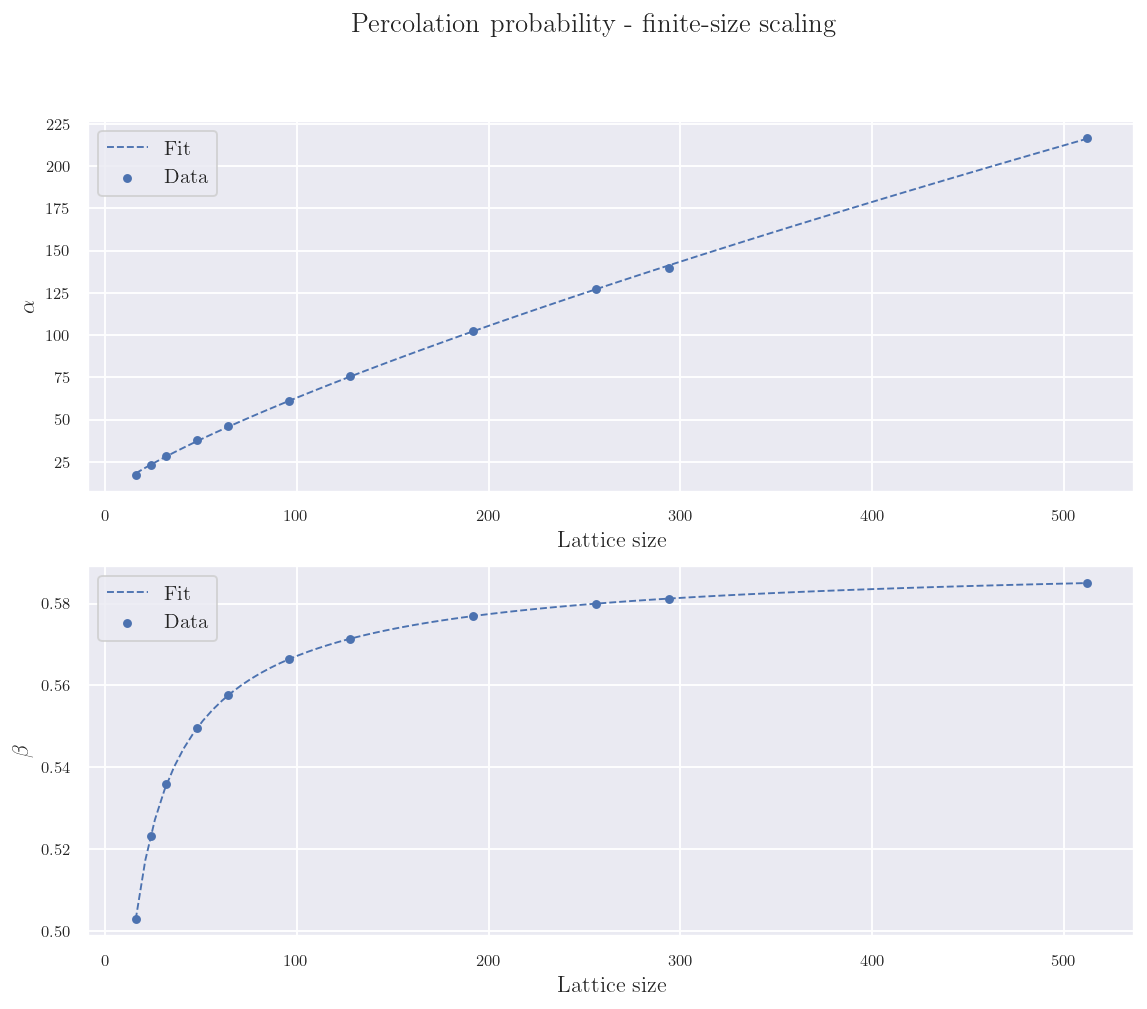
\includegraphics[width=\linewidth]{Images/sec3_perc_prob_3.png}
  \caption{Finite-size scaling analysis of the hyperbolic tangent function}
  \label{fig:sec3_perc_prob_3}
\end{figure}



\section{Percolating cluster strength}


\begin{figure}[H]
  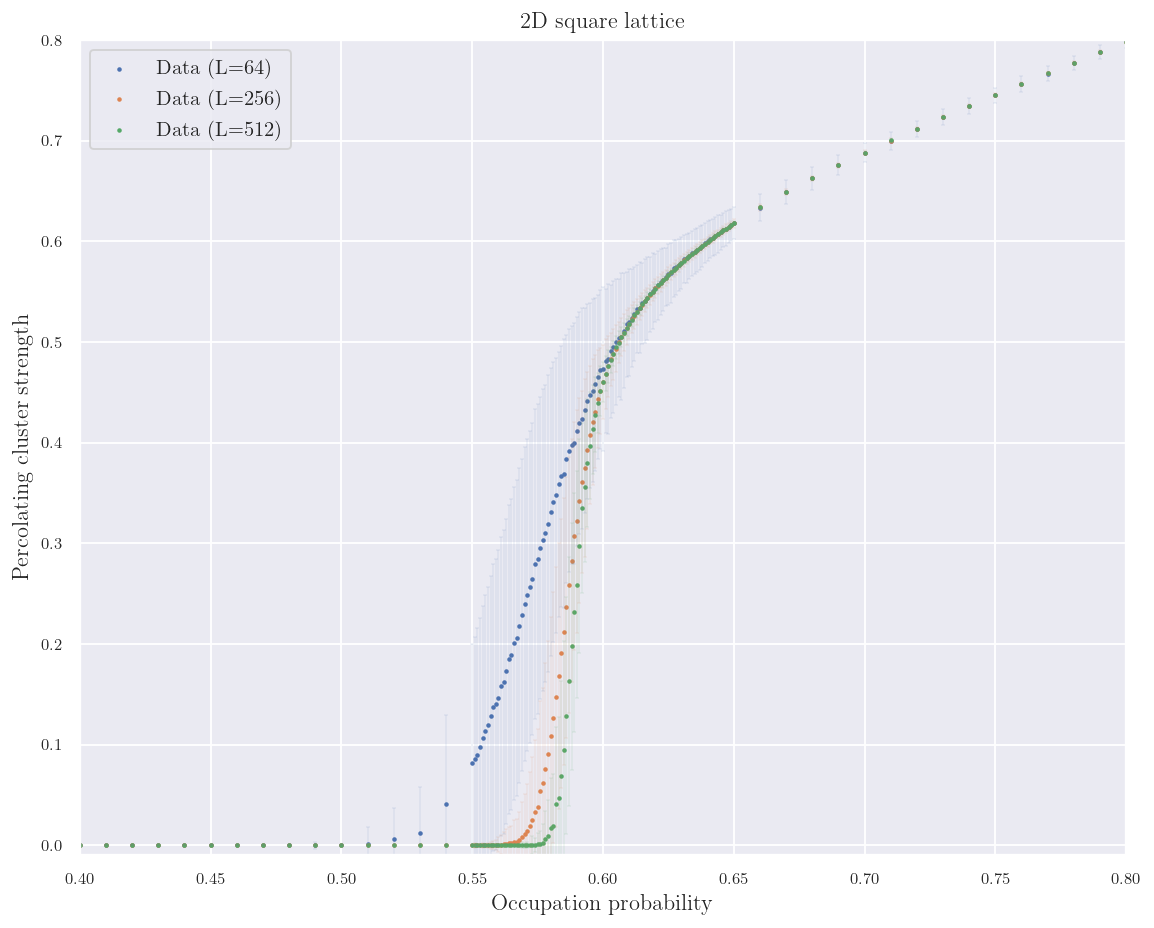
\includegraphics[width=\linewidth]{Images/sec3_perc_clust_strength_1.png}
  \caption{Percolating cluster strength versus occupation probability for various lattice sizes}
  \label{fig:sec3_perc_clust_strength_1}
\end{figure}


\section{Mean cluster size}



\begin{figure}[H]
  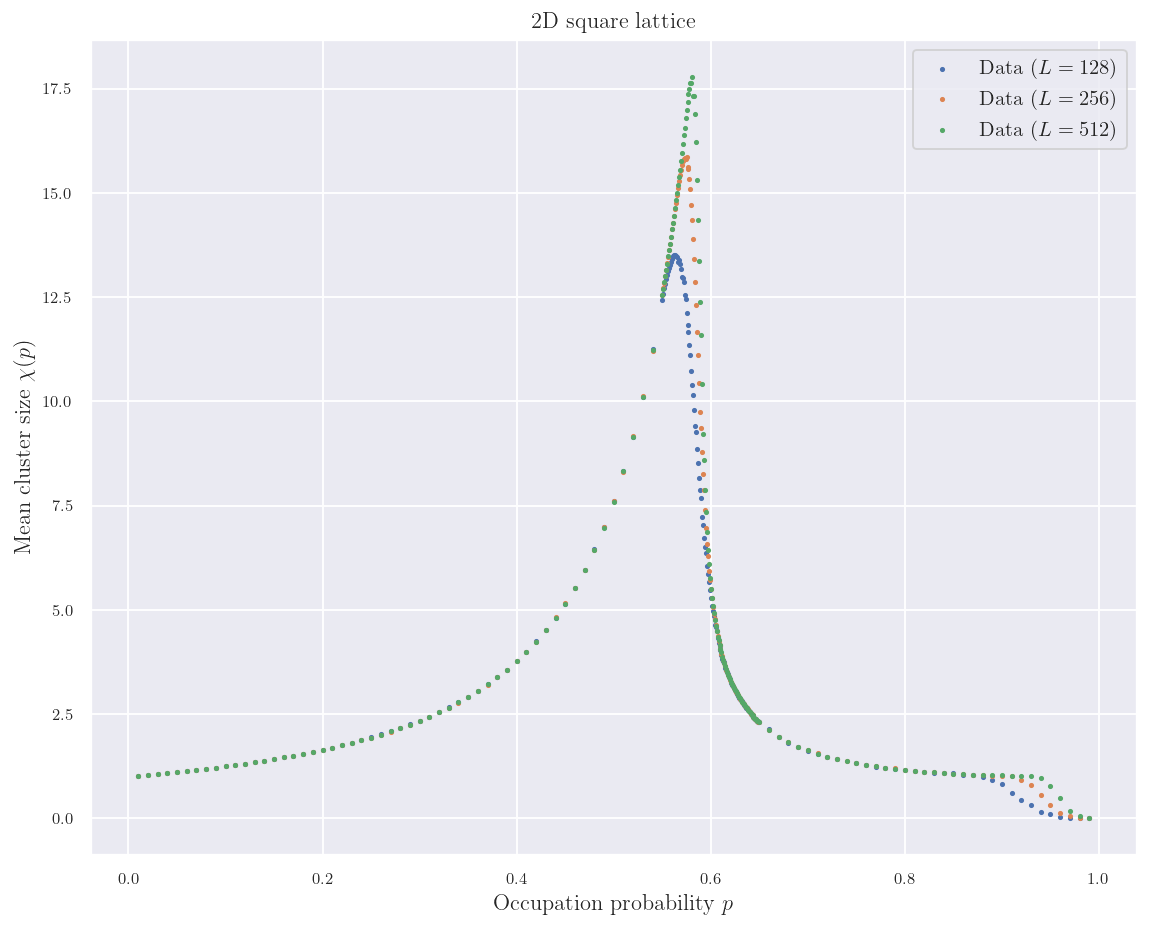
\includegraphics[width=\linewidth]{Images/sec3_mean_cluster_size_1.png}
  \caption{Mean finite cluster size versus occupation probability for various lattice sizes}
  \label{fig:sec3_mean_cluster_size_1}
\end{figure}


\section{Correlation function and correlation length}




\begin{figure}[H]
  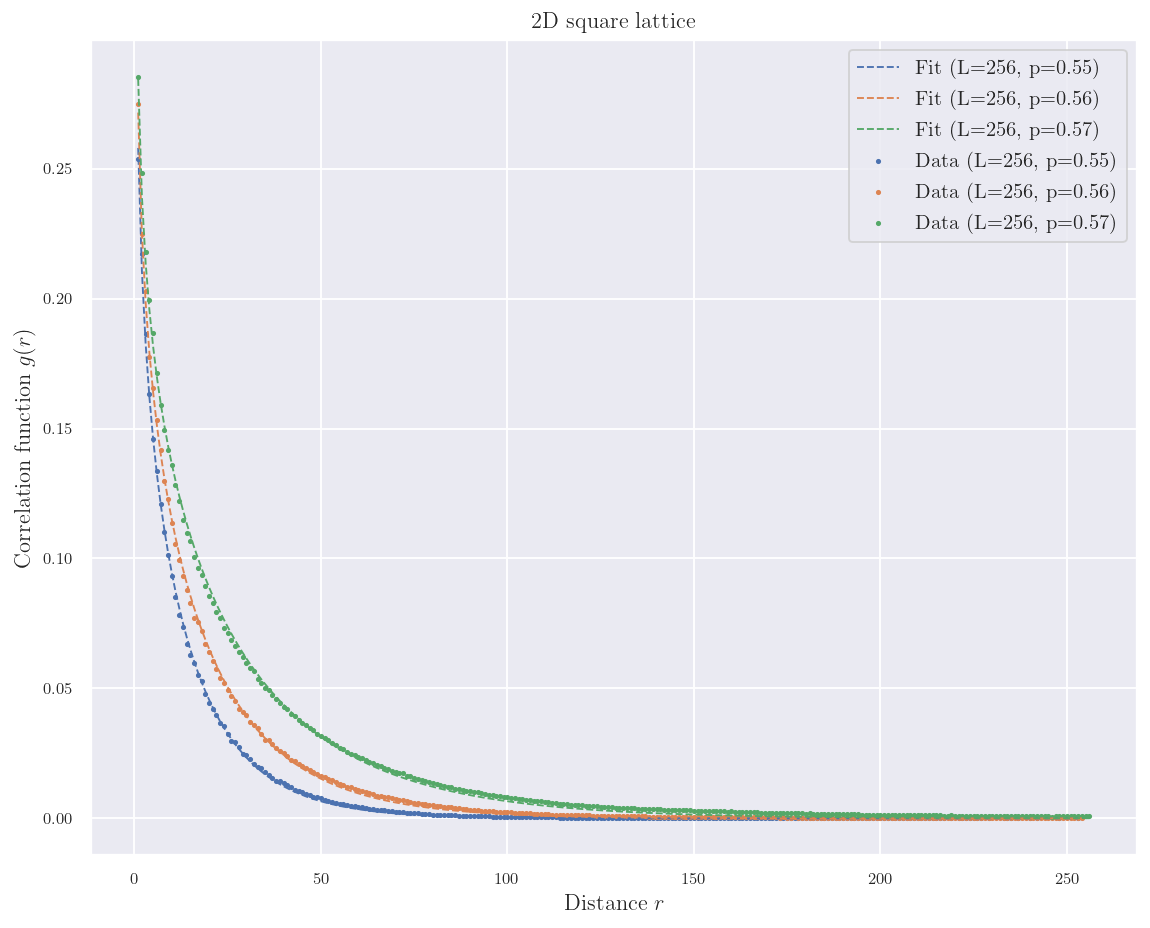
\includegraphics[width=\linewidth]{Images/sec3_corr_func_1.png}
  \caption{Correlation function for various sizes and occupation probabilities}
  \label{fig:sec3_corr_func_1}
\end{figure}


\begin{figure}[H]
  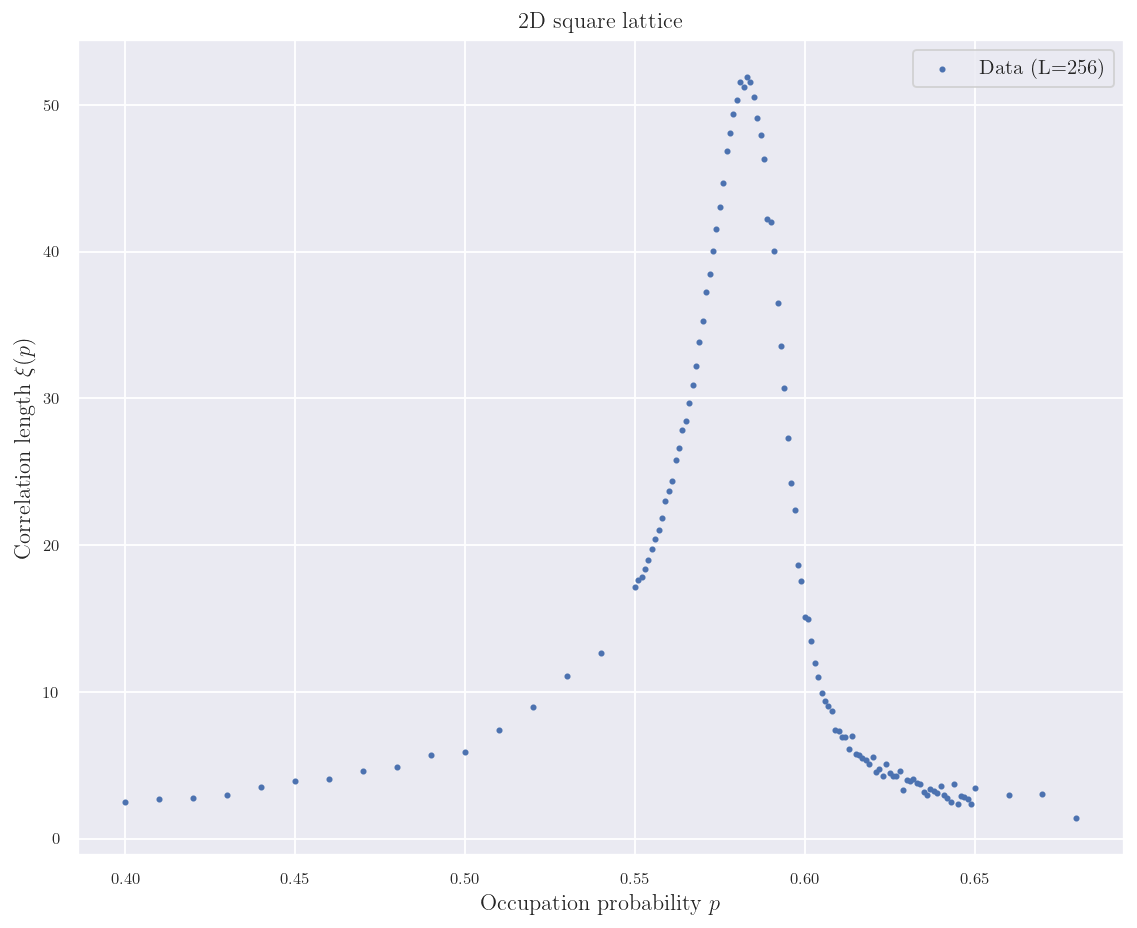
\includegraphics[width=\linewidth]{Images/sec3_corr_length_1.png}
  \caption{Correlation length for multiple lattice sizes}
  \label{fig:sec3_corr_length_1}
\end{figure}




% In 2D percolation, it is normally assumed that $g(r)$ behaves as the product of a power function and a exponential function(REF4), i.e 

$$ 
 g(r) \propto r^{-\nu} e^{-\frac{r}{\xi}}
$$ 
